\documentclass[11pt,a4paper]{article}
\usepackage{ngerman,amssymb,amsmath}

\newif\ifpdf\ifx\pdfoutput\undefined\pdffalse\else\pdfoutput=1\pdftrue\fi

\ifpdf
    \usepackage[pdftex]{graphicx}
    \usepackage[pdftex,colorlinks=true,pdfview=FitB,pdfstartview=FitB, linkcolor=blue, 
            citecolor=blue, urlcolor=blue]{hyperref}

    \pdfinfo{
        /Title (DROPS Manual)
        /Author(Sven Gross, Joerg Peters, Volker Reichelt, Marcus Soemers)
    }
\else
    \usepackage{graphicx}
\fi


\parindent0cm
\parskip1ex
\topmargin-2cm
\oddsidemargin-1cm
\textheight25cm

\textwidth17cm

\newenvironment{Code}{\begin{quote}\scriptsize}{\end{quote}}
\newenvironment{Desc}[3]%
    {\fbox{\Large\tt #1}\qquad#2\hfill{\bf Typ: }{\tt #3}\\[1ex]}%
    {\leavevmode\\[3ex]}

\begin{document}
\newcommand{\prg}[1]{{\tt #1}}

{\Large\bf Eine Sammlung von DROPS aller Geschmacksrichtungen}

\tableofcontents

%============================================================================
\section{{\tt geom}: Geometrie}
%============================================================================

\subsection{Tetraeder und Subsimplices}

Datenstrukturen f"ur die Subsimplices (Knoten, Kanten, Seitenfl"achen) und die
Simplices (Tetraeder): 
\prg{VertexCL}, \prg{EdgeCL}, \prg{FaceCL}, \prg{TetraCL} (siehe
\prg{multigrid.h/cpp}).

Jeder Tetraeder hat Zugriff auf seine 4 Knoten, 6 Kanten und 4 Seitenfl"achen.
Die interne Nummerierung dieser Subsimplices auf einem Tetraeder kann der 
folgenden Skizze entnommen werden:
\begin{figure}[ht!]
\centering
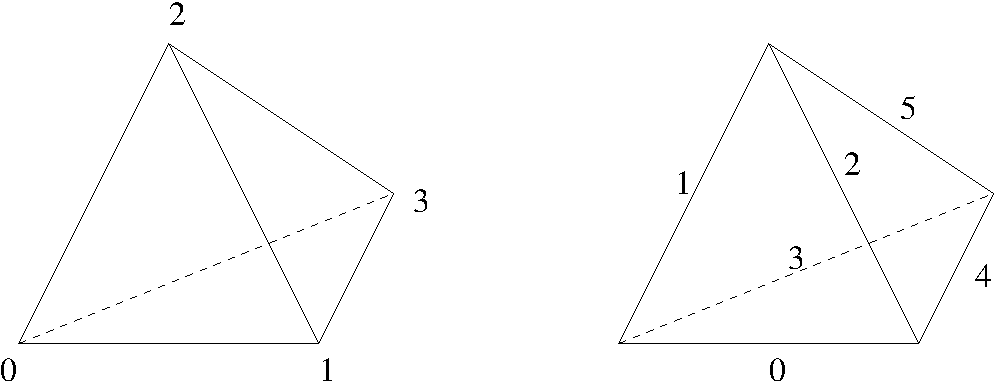
\includegraphics[width=0.5\textwidth]{tetra}
\end{figure}

Die Seitenfl"ache $i$ liegt dem Knoten $i$ gegen"uber. All diese topologischen
Informationen sind in \prg{topo.h/cpp} festgehalten.

\subsection{Das MultiGrid}

Das MultiGrid $\mathcal M$ ist durch die \prg{MultiGridCL} repr"asentiert.
Darin sind die Tetraeder und Subsimplices nach Leveln geordnet abgespeichert.
Das Level eines Objektes gibt gerade die Anzahl seiner Vorfahren an,
entsprechend besitzt das gr"obste Level die Nummer 0. Alle Tetraeder eines
Levels $k$ formen das  sogenannte \emph{Gitter der Stufe $k$}: 
$$
\mathcal G_k=\{T\in\mathcal M: \ell(T)=k\} ~.
$$
Die \emph{Triangulierung der Stufe $k$}
wird vom Gitter $\mathcal G_k$ und allen gr"oberen Tetraedern $T\in\mathcal
G_j, j<k$, die nicht verfeinert sind, gebildet: 
$$
\mathcal T_k:=\mathcal G_k \cup\bigcup_{j<k}\{T\in\mathcal G_j: T\mbox{ ist
unverfeinert}\} ~.
$$


\begin{Code}
\begin{verbatim}
class MultiGridCL
{
    MultiGridCL (const MGBuilderCL& Builder);

    void Refine ();
    void Scale( double);
    void MakeConsistentNumbering();
    void SizeInfo(std::ostream&);
    void ElemInfo(std::ostream&, int Level= -1);

    bool IsSane (std::ostream&, int Level=-1) const;

    VertexIterator         GetVerticesBegin     (int Level);
    VertexIterator         GetVerticesEnd       (int Level);
    AllVertexIteratorCL    GetAllVertexBegin    (int Level=-1);
    AllVertexIteratorCL    GetAllVertexEnd      (int Level=-1);
    TriangVertexIteratorCL GetTriangVertexBegin (int Level=-1);
    TriangVertexIteratorCL GetTriangVertexEnd   (int Level=-1);
    // ... und dasselbe mit const_Iteratoren
    // ... und fuer Edge, Face, Tetra
};
\end{verbatim}
\end{Code}

Der Zugriff auf die Tetraeder und Subsimplices erfolgt "uber entsprechende
Iteratoren, die sich drei Kategorien zuordnen. Am Beispiel der Tetraeder sind
dies:
\begin{itemize}
    \item \prg{TetraIterator} iteriert "uber alle Tetraeder $T\in\mathcal G_k$
    eines Gitters $\mathcal G_k$.
    \item \prg{AllTetraIteratorCL} iteriert "uber alle Tetraeder
    $T\in\bigcup_{j\leq k}{\mathcal G_j}$ bis zum Gitter $\mathcal G_k$.
    \item \prg{TriangTetraIteratorCL} iteriert "uber alle Tetraeder
    $T\in\mathcal T_k$ der Triangulierung $\mathcal T_k$.
\end{itemize}

Der Verfeinerungsalgorithmus wird durch die Elementfunktion \prg{Refine}
aufgerufen und verfeinert alle Tetraeder des MultiGrids $\mathcal M$, die zur
Verfeinerung markiert sind (Ein Tetraeder wird durch Aufruf seiner
Elementfunktion \prg{TetraCL::SetRegRefMark} zur Verfeinerung markiert).

Ein MultiGrid wird mit Hilfe eines \prg{MGBuilderCL}-Objektes erzeugt (siehe
Konstruktor von \prg{MultiGridCL}), welche im n"achsten Abschnitt behandelt
werden.

\subsection{MultiGrid-Builder}
Die Anfangstriangulierung $\mathcal T_0=\mathcal G_0$ wird mit Hilfe einer
Builder-Klasse konstruiert (siehe \verb|geom/builder.h/cpp|). 
Derzeit gibt es in DROPS folgende Builder:
\begin{itemize}
    \item \prg{BrickBuilder} zur Erzeugung eines Quaders.
    \item \prg{LBuilder} zur Erzeugung eines L-Gebietes.
    \item \prg{BBuilder} zur Erzeugung eines B-Gebietes (Quader mit
    einspringender Ecke).
    \item \prg{ReadMeshBuilderCL} liest GAMBIT (FLUENT) Mesh-Files.
\end{itemize}

\begin{Code}
\begin{verbatim}
class BrickBuilderCL : public MGBuilderCL
{
    BrickBuilderCL(const Point3DCL& orig, const Point3DCL& e1, const Point3DCL& e2, const Point3DCL& e3, 
                   Uint n1, Uint n2, Uint n3);
};

class LBuilderCL : public MGBuilderCL
{
    LBuilderCL(const Point3DCL& origin, const Point3DCL& e1, const Point3DCL& e2, const Point3DCL& e3,
               Uint n1, Uint n2, Uint n3, Uint b1, Uint b2);
};

class BBuilderCL : public MGBuilderCL
{
    BBuilderCL(const Point3DCL& origin, const Point3DCL& e1, const Point3DCL& e2, const Point3DCL& e3,
               Uint n1, Uint n2, Uint n3, Uint b1, Uint b2, Uint b3);
};

class ReadMeshBuilderCL : public MGBuilderCL
{
    // Input stream, from which the mesh is read. Pass a pointer to an output stream,
    // e. g. msg= &std::cout, if you want to know, what happens during multigrid-construction.
    ReadMeshBuilderCL(std::istream& f, std::ostream* msg= 0);

    BndCondT GetBC( Uint i)                    const;
    void     GetBC( std::vector<BndCondT>& BC) const;
};
\end{verbatim}
\end{Code}

\subsubsection{\prg{BrickBuilderCL}}
Der Quader wird festgelegt durch den Ursprung \prg{orig}
und die aufspannenden Vektoren \prg{e1, e2, e3}. Der Quader wird dann in
${\mathtt n1}\times{\mathtt n2}\times{\mathtt n3}$ Unterquader zerlegt, von
denen jeder in 6 Tetraeder unterteilt wird.

Die 6 Randsegmente des Quaders werden in folgender Reihenfolge abgespeichert
(als Beispiel der Einheitsw"urfel $\Omega=[0,1]^3$:) 
\begin{itemize}
    \item $x=0, \quad x=1$, 
    \item $y=0, \quad y=1$, 
    \item $z=0, \quad z=1$.
\end{itemize}

\subsubsection{\prg{LBuilderCL}}  Das L-Gebiet wird "ahnlich wie der Quader
festgelegt. Die zus"atzlichen Parameter ${\mathtt b1}<{\mathtt n1}$, ${\mathtt
b2}<{\mathtt n2}$ legen die Aussparung des L-Gebietes fest, welche dem
Ursprung gegen"uber liegt und aus $({\mathtt n1-b1})\times({\mathtt
n2-b2})\times{\mathtt n3}$ Unterquadern besteht.

Die 14 Randsegmente des L-Gebietes werden in folgender Reihenfolge
abgespeichert (als Beispiel das L-Gebiet $\Omega=[0,1]^3\setminus
([0.5,1]^2\times[0,1])$):
\begin{itemize}
    \item $x=0, y\in[0,0.5]$, \quad
    $x=0, y\in[0.5,1]$, \quad
    $x=1, y\in[0,0.5]$, \quad
    $x=0.5, y\in[0.5,1]$,
    \item $y=0, x\in[0,0.5]$, \quad
    $y=0, x\in[0.5,1]$, \quad
    $y=1, x\in[0,0.5]$, \quad
    $y=0.5, x\in[0.5,1]$,
    \item $z=0, (x,y)\in[0,0.5]\times[0,0.5]$, \quad
    $z=0, (x,y)\in[0,0.5]\times[0.5,1]$, \quad
    $z=0, (x,y)\in[0.5,1]\times[0,0.5]$, \\
    $z=1, (x,y)\in[0,0.5]\times[0,0.5]$, \quad
    $z=1, (x,y)\in[0,0.5]\times[0.5,1]$, \quad
    $z=1, (x,y)\in[0.5,1]\times[0,0.5]$.
\end{itemize}
 
\subsubsection{\prg{BBuilderCL}}  Das B-Gebiet wird "ahnlich wie der Quader
festgelegt. Die zus"atzlichen Parameter ${\mathtt b1}<{\mathtt n1}$, ${\mathtt
b2}<{\mathtt n2}$, ${\mathtt b3}<{\mathtt n3}$ legen die Aussparung des
B-Gebietes fest, welche dem Ursprung gegen"uber liegt und aus $({\mathtt
n1-b1})\times({\mathtt n2-b2})\times({\mathtt n3-b3})$ Unterquadern besteht.

Die 24 Randsegmente des L-Gebietes werden in folgender Reihenfolge
abgespeichert (als Beispiel das L-Gebiet $\Omega=[0,1]^3\setminus [0.5,1]^3$):
\begin{itemize}
    \item $x=0, (y,z)\in[0,0.5]\times[0,0.5]$, \quad
    $x=0, (y,z)\in[0,0.5]\times[0.5,1]$, \quad
    $x=0, (y,z)\in[0.5,1]\times[0,0.5]$, \quad
    $x=0, (y,z)\in[0.5,1]\times[0.5,1]$, \\
    $x=1, (y,z)\in[0,0.5]\times[0,0.5]$, \quad
    $x=1, (y,z)\in[0,0.5]\times[0.5,1]$, \quad
    $x=1, (y,z)\in[0.5,1]\times[0,0.5]$, \quad
    $x=0.5, (y,z)\in[0.5,1]\times[0.5,1]$.
    \item analog f"ur die $x$-$z$-Ebene.
    \item analog f"ur die $x$-$y$-Ebene.
\end{itemize}

\subsubsection{\prg{ReadMeshBuilderCL}}
\label{ss:MeshBuilder}
Der Builder versteht das Format des "`User's Guide"' zu TGrid 3, Anhang C, welches
unter anderem von RAMPANT, FLUENT/UNS, TGrid verwendet wird und von dem
Gittergenerator GAMBIT erzeugt wird.
Die ID's der erzeugten Simplices entsprechen denen in der Datei.

Um Randsegmente zu repr"asentieren, wird die Klasse \prg{MeshBoundaryCL} verwendet.
Pro Zone von Randdreiecken in der .msh-Datei wird ein \prg{MeshBoundaryCL}-Objekt
erzeugt, welches die zone-id und die boundary-condition enth"alt (siehe Ahnhang C des
User's Guide).

Zur Erstellung von Gittern mit GAMBIT sei auf die Hinweise in Abschnitt
\ref{s:Gambit} verwiesen.

%============================================================================
\section{{\tt poisson}: Poisson-Gleichung}
%============================================================================

\subsection{station"are Poisson-Gleichung}

Auf dem Gebiet $\Omega$ sei die (verallgemeinerte) Poissongleichung
\[
\begin{array}{rcll}
    -\Delta u(x) + q(x)\cdot u(x) &=& f(x) & \qquad\mbox{in }\Omega\\
    u(x) &=& g_D(x) & \qquad\mbox{auf }\Gamma_D\\
    \frac{\partial u(x)}{\partial n} &=& g_N(x) & \qquad\mbox{auf }\Gamma_N
\end{array}
\]
gegeben, wobei die disjunkten Randst"ucke $\Gamma_D\cup\Gamma_N=\partial\Omega$
den Dirichlet- bzw. Neumannrand darstellen.

F"ur die Finite-Elemente-Diskretisierung mit $P_1$-Elementen steht die
Problemklasse \prg{PoissonP1CL} zur Verf"ugung:
\begin{Code}
\begin{verbatim}
template <class MGB, class Coeff>
class PoissonP1CL: public ProblemCL<MGB, Coeff, PoissonBndDataCL>
{
    IdxDescCL idx;
    VecDescCL x;
    VecDescCL b;
    MatDescCL A;
    
    PoissonP1CL(const MultiGridBuilderCL& mgb, const CoeffCL& coeff, const BndDataCL& bdata);
    // numbering of unknowns
    void CreateNumbering(Uint, IdxDescCL*);
    void DeleteNumbering(IdxDescCL*);
    // set up matrices and rhs
    void SetupSystem         (MatDescCL&, VecDescCL&) const;
    void SetupStiffnessMatrix(MatDescCL&) const;
    void SetupProlongation   (MatDescCL& P, IdxDescCL* cIdx, IdxDescCL* fIdx) const;
    // check computed solution etc.
    double CheckSolution(const VecDescCL&, scalar_fun_ptr) const;
    double CheckSolution(scalar_fun_ptr Lsg) const { return CheckSolution(x, Lsg); }
    void GetDiscError (const MatDescCL&, scalar_fun_ptr) const;
    void GetDiscError (scalar_fun_ptr Lsg) const { GetDiscError(A, Lsg); }

    bool          EstimateError         (const VecDescCL&, const double, double&, est_fun);
    static double ResidualErrEstimator  (const TetraCL&, const VecDescCL&, const BndDataCL&);
    static double ResidualErrEstimatorL2(const TetraCL&, const VecDescCL&, const BndDataCL&);

    DiscSolCL GetSolution() const;
};
\end{verbatim}
\end{Code}

\subsection{instation"are Poisson-Gleichung}
Auf dem Gebiet $\Omega$ sei die instation"are Poissongleichung bzw.
W"armeleitungsgleichung
\[
\begin{array}{rcll}
    \frac{\partial u(x,t)}{\partial t} - \alpha(x,t)\Delta u(x,t) &=& f(x,t) 
    & \qquad\mbox{in }\Omega\times[0,t_f]\\
    u(x,0) &=& u_0(x) & \qquad\mbox{in }\Omega\\
    u(x,t) &=& g_D(x) & \qquad\mbox{auf }\Gamma_D\times[0,t_f]\\
    \alpha(x,t)\frac{\partial u(x,t)}{\partial n} &=& g_N(x) 
    & \qquad\mbox{auf }\Gamma_N\times[0,t_f]
\end{array}
\]
gegeben. Beachte folgende Unterschiede zum station"aren Problem:
\begin{itemize}
  \item Die Temperaturleitf"ahigkeit $\alpha=\frac{\lambda}{\rho c}=\alpha(x,t)$ kann "ortlich und zeitlich variieren und wird in der Diskretisierung der Steifigkeitsmatrix ber"ucksichtigt. Beachte, dass sich dadurch die homogene nat"urliche Randbedingung "andert ($\alpha\frac{\partial u}{\partial n}$ statt $\frac{\partial u}{\partial n}$)!
  \item Der Term $q(x)\cdot u(x,t)$ taucht in der instation"aren Poissongleichung nicht mehr auf (im Gegensatz zur station"aren Gleichung). Die Diskretisierung dieses Terms wurde auskommentiert, da er bislang nicht gebraucht wurde, er kann bei Bedarf aber wieder ber"uchsichtigt werden.
\end{itemize}

\begin{Code}
\begin{verbatim}
\end{verbatim}
\end{Code}

%============================================================================
\section{{\tt stokes}: Stokes-Gleichung}
%============================================================================

\subsection{station"are Stokes-Gleichung}
\begin{Code}
\begin{verbatim}
\end{verbatim}
\end{Code}
\subsection{instation"are Stokes-Gleichung}
\begin{Code}
\begin{verbatim}
\end{verbatim}
\end{Code}
 
%============================================================================
\section{{\tt navstokes}: Navier-Stokes-Gleichung}
%============================================================================
 
\subsection{station"are Navier-Stokes-Gleichung}
\begin{Code}
\begin{verbatim}
\end{verbatim}
\end{Code}
\subsection{instation"are Navier-Stokes-Gleichung}
\begin{Code}
\begin{verbatim}
\end{verbatim}
\end{Code}
 
%============================================================================
\section{{\tt levelset}: Levelset-Methode}
%============================================================================

Die \prg{LevelsetP2CL} implementiert die Funktionalit"at der Levelset-Methode
f"ur $P_2$-Elemente. 

\begin{Code}
\begin{verbatim}
template<class StokesProblemT>
class LevelsetP2CL
{
    LevelsetP2CL( MultiGridCL& mg, double theta= 0.5, double SD= 0.);
    
    void CreateNumbering( Uint level, IdxDescCL*);
    void DeleteNumbering();
    void Init( scalar_fun_ptr);
    // call SetupSystem *before* calling SetTimeStep!
    void SetupSystem( const DiscVelSolCL& vel);
    void SetTimeStep( double dt);
    void DoStep();
    void Reparam( Uint steps, double dt);
    
    bool   Intersects( const TetraCL&) const;
    double GetMass() const;
    static void AccumulateBndIntegral( const MultiGridCL&, VecDescCL& f, const VecDescCL& Phi, double sigma);
    
    DiscSolCL GetSolution() const;
};
\end{verbatim}
\end{Code}

%============================================================================
\section{{\tt num}: Numerik}
%============================================================================

\subsection{Vektoren und d"unnbesetzte Matrizen}

Datentypen f"ur Vektoren und d"unnbesetzte Matrizen sind in der Datei
\verb|num/spmat.h| definiert.

Als Vektordatentyp dient die Template-Klasse \prg{VectorBaseCL<T>}, die direkt
von \prg{std::valarray<T>} abgeleitet ist und so die \emph{expression templates}
der Valarrays ausnutzt. Wenn \prg{DebugNumericC} als Debug-Option gesetzt ist,
findet beim Zugriff auf Vektoreintr"age mit \prg{[]} sowie bei Benutzung der
Operatoren \prg{+, -, =, +=, -=, *=, /=} eine Bereichspr"ufung statt (im Gegensatz zum reinen
valarray). Folgende Funktionen sind f"ur Vektoren definiert:
\begin{itemize}
  \item \prg{dot(x,y)} berechnet das Skalarprodukt $x^T y$,
  \item \prg{norm(x)} berechnet die euklidische Norm $\|x\|_2$, 
    \verb|norm_sq(x)| dessen Quadrat $\|x\|_2^2$,
  \item \prg{supnorm(x)} berechnet die Maximumsnorm $\|x\|_\infty$,
  \item \verb|axpy(a,x,y)| f"ur \verb|y+= a*x|,
  \item \verb|z_xpay(z,x,a,y)| f"ur \verb|z= x + a*y|,
  \item \verb|z_xpaypby2(z,x,a,y,b,y2)| f"ur \verb|z= x + a*y + b*y2|.
\end{itemize}

Die d"unnbesetzten Matrizen werden in einem zeilenbasierten Format gespeichert
und durch folgende Template-Klasse realisiert:

\begin{Code}
\begin{verbatim}
template <typename T>
class SparseMatBaseCL
{
    SparseMatBaseCL (size_t rows, size_t cols, size_t nz);

    size_t num_rows     () const;
    size_t num_cols     () const;
    size_t num_nonzeros () const;

    inline T  operator() (size_t i, size_t j) const;
    SparseMatBaseCL& operator*= (T c);
    SparseMatBaseCL& operator/= (T c);
    SparseMatBaseCL& LinComb (double, const SparseMatBaseCL<T>&,
                              double, const SparseMatBaseCL<T>&);
    void clear();
};
\end{verbatim}
\end{Code}
Mit Hilfe der Funktion \verb|LinComb| wird die Matrix als Linearkombination
zweier anderer Matrizen erzeugt (interessant bei der Zeitintegration: $\frac{1}{dt}M+\theta
A$). Die Funktion \verb|clear| dagegen l"oscht den Inhalt der Matrix.

Matrix-Vektor-Multiplikation erfolgt mit \verb|A*x| f"ur $Ax$ 
und \verb|transp_mul(A,x)| f"ur $A^Tx$.

Da das \emph{sparsity pattern} einer Matrix vorher meist nicht bekannt ist, wird
beim Aufstellen der Matrizen zun"achst ein Zwischenformat, die
\verb|SparseMatBuilderCL| erzeugt, in der das \emph{sparsity pattern} aufgebaut
wird, bevor schlie"slich die endg"ultige Matrix mit dem Befehl \verb|Build|
erzeugt wird. 
\begin{Code}
\begin{verbatim}
template <typename T>
class SparseMatBuilderCL
{
    SparseMatBuilderCL(spmatT* mat, size_t rows, size_t cols);

    T& operator() (size_t i, size_t j);
    void Build();
};
\end{verbatim}
\end{Code}
Besitzt die an den Builder "ubergebene Matrix bereits ein \emph{sparsity
pattern}, so wird dieses aus Effizienzgr"unden wiederverwendet. Deswegen sollte
nach jeder Gitter"anderung der Inhalt der Matrizen mit \verb|clear| gel"oscht
werden, um das \emph{sparsity pattern} neu aufbauen zu lassen.

Zur einfacheren Handhabung sind die folgenden typedefs definiert:
\begin{Code}
\begin{verbatim}
typedef VectorBaseCL<double>       VectorCL;
typedef SparseMatBaseCL<double>    MatrixCL;
typedef SparseMatBuilderCL<double> MatrixBuilderCL;
\end{verbatim}
\end{Code}


\subsection{Vorkonditionierer}
\label{ss:vorkonditionierer}
Die Vorkonditionierer f"ur ein lineares Gleichungssystem $Ax=b$ sind
in \prg{num/solver.h} definiert. Sie haben im wesentlichen die folgende
Struktur:
\begin{Code}
\begin{verbatim}
template <PreMethGS PM>
class PreGSCL<PM, false>
{
  private:
    double _omega;

  public:
    PreGSCL (double om= 1.0) : _omega(om) {}

    template <typename Vec>
    void Apply(const MatrixCL& A, Vec& x, const Vec& b) const
};
\end{verbatim}
\end{Code}
Die Funktion \prg{Apply} wendet den Vorkonditionierer an. Zur Zeit gibt
es folgende Verfahren:
\begin{itemize}
\item \prg{SORsmoothCL}, Gauss-Seidel-Verfahren mit "Uberrelaxation.
\item \prg{SGSPcCL}, symmetrisches Gauss-Seidel-Verfahren f"ur den Startvektor $x=0$. 
\item \prg{SSORPcCL}, SSOR-Verfahren f"ur den Startvektor $x=0$.
\item \prg{SSORDiagPcCL}, SSOR-Verfahren, f"ur schnelleren Zugriff auf die Diagonale von $A$ optimiert.
\item \prg{DummyPcCL}, die Identit"at als trivialer Vorkonditionierer.
\end{itemize}
Ferner existiert die Funktion \prg{SolveGSstep(const
PreDummyCL<PB\_JAC>\&, const MatrixCL\& A, Vec\& x, const Vec\& b, double
omega)}, die einen Jacobi-Schritt zum Startvektor $x$ durchf"uhrt. Der
Funktionsname ist durch die Auswahlregeln f"ur "uberladene Funktionen
in C++ bedingt.

Die eigentliche Information "uber den Typ des Vorkonditionierers steckt in
\prg{enum PreMethGS} bzw.\ der Template-Klasse 
\verb|template <PreBaseGS> class PreDummyCL {}|, die die \prg{enum}-Werte 
auf eigene C++-Typen abbildet.

\subsubsection{Vorkonditionierer f"ur die station"aren Stokes-Gleichungen}
In \prg{stokes/sdropsP2.cpp} befindet sich die Klasse
\begin{Code}
\begin{verbatim}
class MGPreCL
{
    MGPreCL( const MGDataCL& mgd, const MatrixCL& ps);

    template <typename Mat, typename Vec>
    void
    Apply(const Mat& K, Vec& x, const Vec& b) const;
};
\end{verbatim}
\end{Code}
Sie implementiert einen Blockdiagonal-Vorkonditionierer f"ur die
station"aren Stokes-Gleichungen.  Die Argumente x, b von \prg{Apply}
m"ussen Zugriff auf die Gechwindigkeitskomponenten erm"oglichen (via
der Elementfunktion \prg{u}) und ebenso auf die Druckkomponenten (via
\prg{p}). Dies leistet im Moment die Vektorklasse \prg{StokesVectorCL},
welche in \prg{stokes/sdropsP2.cpp} definiert ist.

Die Matrix K repr"asentiert die Block-Matrix zu den Stokes-Gleichungen
und mu"s Zugriff auf die Teilmatrizen A und B erlauben. Zur Zeit die
in \prg{stokes/sdropsP2.cpp} definierte Klasse \prg{StokesMatrixCL}
eingesetzt.

Der Vorkonditionierer verwendet f"ur den Poissonanteil der
Stokes-Gleichungen eine Iteration des "ubergebenen Mehrgitter-V-Zyklus
mit den in diesem eingestellten Gl"attern.

Die Schur-Komplementmatrix wird durch einen SSOR-Schritt mit der
$P_2$-Massenmatrix vorkonditioniert.

\medskip
Als traditionelle Alternative kann ein "ahnlicher aufgebauter
Vorkonditionierer vom Typ
\begin{Code}
\begin{verbatim}
class FullPreCL
{
    FullPreCL( const MatrixCL& ps);

    template <typename Mat, typename Vec>
    void
    Apply(const Mat& K, Vec& x, const Vec& b) const;
};
\end{verbatim}
\end{Code}
verwendet werden. Im Unterschied zu \prg{MGPreCL} wird hier der
Poissonanteil mit Hilfe eines SSOR-vorkonditionierten PCG-L"osers
n"aherungsweise gel"ost.\footnote{Diese Klasse ist viel ineffizienter
als \prg{MGPreCL}.}

\medskip
Beide Vorkonditionierer liefern bereits korrekte Ergebnisse. Die Implementierung
hat sich jedoch in Details noch nicht stabilisiert. Deshalb befindet sich der
gesamte Code in \prg{stokes/sdropsP2.cpp}.

\subsection{Poisson-L"oser}
Die iterativen L"oser f"ur lineare Gleichungssysteme sind in
\prg{num/solver.h} implementiert.  Es gibt einen CG-L"oser,
\begin{Code}
\begin{verbatim}
template <typename Mat, typename Vec>
bool
CG(const Mat& A, Vec& x, const Vec& b, int& max_iter, double& tol),
\end{verbatim}
\end{Code}
einen PCG-L"oser, der die in \ref{ss:vorkonditionierer} beschriebenen Vorkonditionierer
verwenden kann:
\begin{Code}
\begin{verbatim}
template <typename Mat, typename Vec, typename PreCon>
bool
PCG(const Mat& A, Vec& x, const Vec& b, const PreCon& M,
    int& max_iter, double& tol),
\end{verbatim}
\end{Code}
Ein MINRES-L"oser
\begin{Code}
\begin{verbatim}
template <typename Mat, typename Vec>
bool
MINRES(const Mat& A, Vec& x, const Vec& rhs, int& max_iter, double& tol);
\end{verbatim}
\end{Code}
und ein vorkonditionierter PMINRES-L"oser
\begin{Code}
\begin{verbatim}
template <typename Mat, typename Vec, typename Lanczos>
bool
PMINRES(const Mat& A, Vec& x, const Vec& rhs, Lanczos& q, int& max_iter, double& tol);
\end{verbatim}
\end{Code}
stehen zur Verf"ugung. Sie k"onnen auch direkt
zum L"osen der Stokes-Gleichungen verwendet werden. Beispiele dazu findet man in
\prg{stokes/sdropsP2}.

Ferner existiert eine GMRES-Implementierung:
\begin{Code}
\begin{verbatim}
template <typename Mat, typename Vec, typename PreCon>
bool
GMRES(const Mat& A, Vec& x, const Vec& b, const PreCon& M,
      int m, int& max_iter, double& tol).
\end{verbatim}
\end{Code}
Um die Handhabung der L"oser zu erleichtern gibt es die Klasse
\begin{Code}
\begin{verbatim}
class SolverBaseCL
{
  protected:
    int    _maxiter, _iter;
    double _tol, _res;

    SolverBaseCL (int maxiter, double tol)
        : _maxiter(maxiter), _iter(-1), _tol(tol), _res(-1.) {}

  public:
    void   SetTol    (double tol) { _tol= tol; }
    void   SetMaxIter(int iter)   { _maxiter= iter; }

    double GetTol    () const { return _tol; }
    int    GetMaxIter() const { return _maxiter; }
    double GetResid  () const { return _res; }
    int    GetIter   () const { return _iter; }
},
\end{verbatim}
\end{Code}
welche als Basisklasse f"ur die iterativen L"oser dient. Die abgeleiteten
Klassen enthalten die Elementfunktion \prg{Solve}. Diese ruft den
eigentlichen L"oser mit den vorher gew"ahlten Parametern auf.

\subsection{Stokes-L"oser}
Die Stokes-L"oser ermitteln die L"osung eines linearen Gleichungssystems der Form
$$
\begin{pmatrix}A & B^T \\ B & 0\end{pmatrix}
\begin{pmatrix}u \\ p\end{pmatrix}
=
\begin{pmatrix}b \\ c\end{pmatrix}.
$$
Sie sind in \prg{num/stokessolver.h} implementiert.

\subsubsection{Schur-Verfahren}
Die Schur-Komplementmatrix $S=BA^{-1}B^T$ wird in Drops durch die Klasse
\prg{SchurComplMatrixCL} in \prg{stokes/stokes.h} realisiert. Der Matrix-Vektor-Multiplikationsoperator
verwendet zu L"osung des Gleichungssystems mit $A$ ein PCG-Verfahren mit dem
in der \prg{SchurComplMatrixCL} definierten Vorkonditionierer. Dies ist gegenw"artig
die \prg{SSORPcCL}.

Damit kann das Schur-Verfahren in \prg{SchurSolverCL} und \prg{PSchurSolverCL} so
darstellen:
\begin{enumerate}
\item $r= BA^{-1}b -c$ berechnen: \quad $r= -c$, $Av = b$ l"osen, $r+= Bv$.
\item $Sp=r$ l"osen.
\item $Av = b - B^Tp$ l"osen.
\end{enumerate}
Beide Klassen verwenden in Schritt 1 und 3 einen der Poissonl"oser,
dessen Typ als Template-Parameter in die Klasse gebracht wird (H"alt
eine Referenz auf den L"oser.). Ein Objekt vom L"osertyp wird
erst durch "offentliches Ableiten zugef"ugt. In Schritt 2 verwendet
\prg{SchurSolverCL} das CG-Verfahren und \prg{PSchurSolverCL} ein
PCG-Verfahren mit SSOR-Vorkonditionierung einer Matrix in den Druckunbekannten 
(z.\,B. Massenmatrix).

Zur einfacheren Handhabung werden folgende abgeleiteten Klassen bereitgestellt:
\begin{Code}
\begin{verbatim}
class Schur_PCG_CL: public SchurSolverCL<PCG_SsorCL>
{
    Schur_PCG_CL(int outer_iter, double outer_tol, int inner_iter, double inner_tol);
};


class PSchur_PCG_CL: public PSchurSolverCL<PCG_SsorCL>
{
    PSchur_PCG_CL( MatrixCL& M, int outer_iter, double outer_tol, int inner_iter, double inner_tol);
};


class PSchur_IPCG_CL: public PSchurSolverCL<PCG_SsorDiagCL>
{
    PSchur_IPCG_CL( MatrixCL& M, int outer_iter, double outer_tol, int inner_iter, double inner_tol);
};


class PSchur_GSPCG_CL: public PSchurSolverCL<PCG_SgsCL>
{
    PSchur_GSPCG_CL( MatrixCL& M, int outer_iter, double outer_tol, int inner_iter, double inner_tol);
};


class PSchur_MG_CL: public PSchurSolverCL<MGSolverCL>
{
    PSchur_MG_CL( MatrixCL& M,      int outer_iter, double outer_tol, 
                  MGDataCL& MGData, int inner_iter, double inner_tol );
};
\end{verbatim}
\end{Code}


\subsubsection{Uzawa-Verfahren}
Die folgenden Uzawa-Verfahren stehen zur Verf"ugung:
\begin{Code}
\begin{verbatim}
template <typename PoissonSolverT>
class UzawaSolverCL : public SolverBaseCL
{
    UzawaSolverCL (PoissonSolverT& solver, MatrixCL& M, int maxiter, double tol, double tau= 1.);

    void Solve( const MatrixCL& A, const MatrixCL& B, VectorCL& v, VectorCL& p,
                const VectorCL& b, const VectorCL& c);
// ...
};

class Uzawa_IPCG_CL : public SolverBaseCL
{
    Uzawa_IPCG_CL(MatrixCL& M, int outer_iter, double outer_tol, int inner_iter, double inner_tol, double tau= 1.);

    // Always call this when A has changed, before Solve()!
    void Init_A_Pc(MatrixCL& A) { _A_IPCGsolver.GetPc().Init(A); }

    inline void Solve( const MatrixCL& A, const MatrixCL& B, VectorCL& v, VectorCL& p,
                       const VectorCL& b, const VectorCL& c);
// ...
};
\end{verbatim}
\end{Code}

In der ersten Klasse ist der Typ des Poissonl"osers als Template-Parameter gegeben.
F"ur die in DROPS vorhandenen Poisson-Verfahren existieren in \prg{num/stokessolver.h}
von \prg{UzawaSolverCL} abgeleitete Klassen, die den entsprechenden L"oser in den
im folgenden Algorithmus auftretenden Poisson-Problemen einsetzen:
\begin{enumerate}
\item $M dp = (B v -c)$ l"osen.
\item $p += dp$.
\item $A dv = A v + B^Tp - b$ l"osen.
\item $v-= dv$.
\end{enumerate}
In der Klasse \prg{Uzawa\_IPCG\_CL} k"onnen in Schritt 1 und 3
unterschiedliche Poisson-Verfahren benutzt werden. Zur Zeit sind beide
L"oser SSOR-vorkonditionierte PCG-Verfahren.

Zur einfacheren Handhabung werden folgende abgeleiteten Klassen bereitgestellt:
\begin{Code}
\begin{verbatim}
class Uzawa_CG_CL : public UzawaSolverCL<CGSolverCL>
{
    Uzawa_CG_CL( MatrixCL& M, int outer_iter, double outer_tol, int inner_iter, double inner_tol, double tau= 1.);
};

class Uzawa_PCG_CL : public UzawaSolverCL<PCG_SsorCL>
{
    Uzawa_PCG_CL( MatrixCL& M, int outer_iter, double outer_tol, int inner_iter, double inner_tol, double tau= 1.);
};

class Uzawa_SGSPCG_CL : public UzawaSolverCL<PCG_SgsCL>
{
    Uzawa_SGSPCG_CL( MatrixCL& M, int outer_iter, double outer_tol, int inner_iter, double inner_tol, double tau= 1.);
};

class Uzawa_MG_CL : public UzawaSolver2CL<PCG_SsorCL, MGSolverCL>
{
    Uzawa_MG_CL(MatrixCL& M,      int outer_iter, double outer_tol,
                MGDataCL& MGData, int inner_iter, double inner_tol, double tau= 1.);
};
\end{verbatim}
\end{Code}

\subsection{Navier-Stokes-L"oser}
Im\prg{num/nssolver.h} sind die L"osungsverfahren f"ur die station"aren
Navier-Stokes-Gleichungen definiert. Sie l"osen das nicht-lineare
Gleichungssystem
$$
\begin{pmatrix}A +\alpha N(v) & B^T p \\ B & 0\end{pmatrix}
\begin{pmatrix}v \\ p\end{pmatrix} = \begin{pmatrix}b \\ c\end{pmatrix}.
$$
Der Parameter $\alpha$ ist hier stets $1$, wird jedoch f"ur die
Zeitintegration ben"otigt. In DROPS wird ein Fixpunktverfahren eingesetzt,
in dem folgende Schritte bis zur Konvergenz iteriert werden:
\begin{enumerate}
\item Stelle $N(v)$ auf.
\item L"ose
$$
\begin{pmatrix}A + \alpha N(v) & B^T \\ B & 0\end{pmatrix}
\begin{pmatrix}w \\ q\end{pmatrix}
=
\begin{pmatrix}(A +\alpha N(v)) v + B^T p - b\\ B v - c\end{pmatrix}.
$$
\item $v-=w$, $p-=q$.
\end{enumerate}

Die Implementierung findet man in der Klasse \prg{FixedPtDefectCorrCL},
deren abgeleitete Klassen konkrete Stokes-L"oser aus
\prg{num/stokessolver.h} verwenden.

Nach Turek (Seite 187 ff.) kann man obige Defektkorrektur
d"ampfen. Diese Variante des Fixpunktverfahrens wird durch die Klasse
\prg{AdaptFixedPtDefectCorrCL} implementiert.

%============================================================================
\section{Zeitintegration}
%============================================================================
Die Verfahren zur L"osung zeitabh"angiger Gleichungen befinden
sich in der Erprobung und haben noch keinen festen Platz in der
DROPS-Verzeichnishierarchie.  In \prg{poisson}, \prg{stokes} und
\prg{navstokes} gibt es je eine Datei \prg{integrtime.h}, die stets ein
Theta-Schema enth"alt.

\subsection{$\theta$-Schema}
Diese Verfahren ergeben sich dadurch, da"s man in der gew"ohnlichen Differentialgleichung
\[
  u_t = F(u)
\]
die Terme durch folgende Approximationen ersetzt:
$$
  u_t \approx \frac{(1-\theta) u^\text{alt} + \theta u^\text{neu}}{dt}
$$
sowie
\[
  F(u) \approx (1-\theta) F(u^\text{alt}) + \theta F(u^\text{neu}).
\]
Man erh"alt f"ur
jeden Zeitschritt ein (nicht-) lineares Gleichungssystem. Bei den Stokes-
bzw.\ Navier-Stokes-Gleichungen wird der Druck stets vollimplizit
diskretisiert.  Auf diese Weise wird die Berechnung eines Startwertes
f"ur den Druck vermieden.

Die Klassen \prg{Instat***ThetaSchemeCL} enthalten eine Funktion
\prg{SetTimeStep}, die vor jedem Zeitschritt aufgerufen werden mu"s. Sie
stellt das Gleichungssystem mit der Massenmatrix auf und setzt die
Zeitschritt-Gr"o"se.  Der eigentliche Zeitschritt wird durch einen Aufruf
von \prg{DoStep} durchgef"uhrt.

\subsection{Fractional-Step-Verfahren}
F"ur die Stokes-Gleichungen ist ein weiteres Verfahren verf"ugbar:
(XXX beschreiben. Ist im Moment defekt...)

%============================================================================
\section{{\tt out}: Ausgabe}
%============================================================================

\subsection{Ausgabe in Geomview}
\begin{itemize}
    \item \prg{GeomMGOutCL}: nur Triangulierung ausgeben.
    \item \prg{GeomSolOutCL}: Triangulierung ausgeben, die nach den Werten 
    einer skalaren Variable eingef"arbt ist.
\end{itemize}

\begin{Code}
\begin{verbatim}
class GeomMGOutCL : public MGOutCL
{
    GeomMGOutCL (const MultiGridCL& MG, int TriLevel=-1, bool onlyBnd=false, double explode=0.5);
};

template <class DiscSol>
class GeomSolOutCL : public MGOutCL
{
    GeomSolOutCL (const MultiGridCL& MG, const DiscSol& discsol, const ColorMapperCL* colmap, int TriLevel=-1, 
                  bool onlyBnd=false, double explode=0.5, double min=0., double max=1.);
};
\end{verbatim}
\end{Code}

Mit \prg{onlyBnd=true} werden nur die am Rand liegenden Tetraeder ausgegeben
(schnellerer Aufbau von Postscript-Bildern!). "Uber den Parameter \prg{explode}
kann der Versatz der Tetraeder untereinander gesteuert werden, bei
\prg{explode=0} ist dieser Effekt ausgeschaltet. Die Parameter \prg{min, max}
geben an, ab welchen Grenzen die Werte der dargestellten L"osung geclippt
werden sollen.

Die Geomview-Ausgabe ist vor allem f"ur die Ausgabe der Geometrie und
Triangulierung geeignet. Um L"osungen zu betrachten, sollten die folgende
TecPlot- (f"ur 2D-Daten) oder Ensight-Ausgabe (f"ur 3D-Daten) genutzt werden.

\subsection{Ausgabe in TecPlot}
\begin{itemize}
    \item \prg{TecPlot2DSolOutCL}: Ausgabe von Druck und Geschwindigkeit 
    in einer Schnittebene senkrecht zu einer der Koordinatenachsen.
    \item \prg{TecPlotSolOutCL}: Ausgabe von Druck und Geschwindigkeit im gesamten
    Gebiet. Da Tecplot zur 3D-Visualisierung nicht so geeignet ist, empfiehlt
    sich anstattdessen eine Ausgabe f"ur Ensight!
\end{itemize}

\begin{Code}
\begin{verbatim}
template <class DiscVelT, class DiscPrT>
class TecPlot2DSolOutCL: public MGOutCL
{
    TecPlot2DSolOutCL( const MultiGridCL& mg, const DiscVelT& v, const DiscPrT& p, 
                       const IdxDescCL& freeVertIdx, int lvl, Uint cutvar, double cutplane);
};

template <class DiscVelT, class DiscPrT>
class TecPlotSolOutCL: public MGOutCL
{
    TecPlotSolOutCL( const MultiGridCL& mg, const DiscVelT& v, const DiscPrT& p, int lvl= -1);
};
\end{verbatim}
\end{Code}
Die Klasse \prg{TecPlot2DSolOutCL} ben"otigt zur Nummerierung der Knoten einen 
Index, in dem alle $P_1$-Freiheitsgrade durchnummeriert sind. Dieser wird nicht
ver"andert, es kann also z.B. auch der Index der Druckvariable hierzu benutzt
werden. Hier ein Beispiel zur Benutzung:
\begin{Code}
\begin{verbatim}
DROPS::IdxDescCL tecIdx;
tecIdx.Set( 1);
Stokes.CreateNumberingPr( mg.GetLastLevel(), &tecIdx);    

std::ofstream v2d("data2D.dat");
DROPS::TecPlot2DSolOutCL< MyStokesCL::DiscVelSolCL, MyStokesCL::DiscPrSolCL>
    tecplot2d( mg, prob.GetVelSolution(), prob.GetPrSolution(), tecIdx, -1, 1, 0.5); // cutplane is y=0.5
v2d << tecplot2d;
v2d.close();
\end{verbatim}
\end{Code}

\subsection{Ausgabe in Ensight}
\prg{EnsightP2SolOutCL}: Ausgabe im Ensight-Case-Format, auch transiente Daten
m"oglich.
\begin{Code}
\begin{verbatim}
class EnsightP2SolOutCL
{
    EnsightP2SolOutCL( const MultiGridCL& mg, const IdxDescCL* idx, bool binary=true);
    // call CaseBegin() before any other member function
    void CaseBegin ( const char casefileName[], Uint numsteps= 0);
    void DescribeGeom  ( const char geoName[], std::string fileName, bool timedep= false);
    void DescribeScalar( const char varName[], std::string fileName, bool timedep= false);
    void DescribeVector( const char varName[], std::string fileName, bool timedep= false);
    void putGeom      ( std::string, double t= -1);
    template<class DiscScalT>
    void putScalar    ( std::string, const DiscScalT&, double t= -1);
    template<class DiscVecT>
    void putVector    ( std::string, const DiscVecT&, double t= -1);
    void Commit    ();    // rewrites case file
    // call CaseEnd() after finishing all other output
    void CaseEnd   ();
};
\end{verbatim}
\end{Code}

Die Klasse \prg{EnsightP2SolOutCL} ben"otigt einen eigenen Index, in dem alle
$P_2$-Freiheitsgrade durchnummeriert sind. Die Aufrufe von Elementfunktionen
werden durch \prg{CaseBegin} am Anfang und \prg{CaseEnd} am Ende
eingeschlossen. Beachte, dass das Case-File in der Regel fehlerhaft sein
wird, wenn \prg{CaseEnd} nicht aufgerufen wird. Die Funktionen
\prg{DescribeXXX} dienen zur Beschreibung der Geometrie und skalarer oder
vektorwertiger Variablen und werden einmal zu Anfang aufgerufen. Der Parameter
\prg{timedep} gibt dabei an, ob es sich um transiente Daten handelt. Mit den
Funktionen \prg{putXXX} k"onnen die Daten dann tats"achlich abgespeichert
werden. Bei transienten Daten muss dabei noch der entsprechende Zeitpunkt
angegeben werden. 
Sind alle Daten f"ur einen Zeitschritt geschrieben, so sollte 
\prg{Commit} aufgerufen werden, um den Zeitschritt im case-file eintragen zu lassen. 
Somit k"onnen die bereits berechneten Zeitschritte visualisiert werden, w"ahrend die 
"ubrige Rechnung noch l"auft. Die Daten werden standardm"a"sig im bin"aren Format 
abgespeichert, durch Setzen des entsprechenden Konstruktorparameters \prg{binary}
kann auch auf ASCII-Ausgabe umgeschaltet werden.

Hier ein Beispiel zur Ausgabe von transienten skalaren Daten bei festem Gitter
und festem Geschwindigkeitsfeld:
\begin{Code}
\begin{verbatim}
IdxDescCL lidx;
lidx.Set( 1, 1);
lset.CreateNumbering( mg.GetLastLevel(), &lidx);
EnsightP2SolOutCL ensight( mg, &lidx);

const char datgeo[]= "ensight/drop.geo", 
           datvec[]= "ensight/drop.vec",
           datscl[]= "ensight/drop.scl";

ensight.CaseBegin     ( "drop.case", num_steps+1);
ensight.DescribeGeom  ( "rotating vel field", datgeo);
ensight.DescribeScalar( "Levelset", datscl, true); 
ensight.DescribeVector( "Velocity", datvec); 

ensight.putGeom( datgeo);
ensight.putVector( datvec, prob.GetVelSolution());
ensight.putScalar( datscl, lset.GetSolution(), 0);

for (int i=1; i<=num_steps; ++i)
{
    // berechne Loesung zum neuen Zeitschritt
    // ...
    ensight.putScalar( datscl, lset.GetSolution(), i/10.);
    ensight.Commit();
}

ensight.CaseEnd();
\end{verbatim}
\end{Code}

\subsection{Einlesen von bereits berechneten Daten im Ensight-Format}
\prg{ReadEnsightP2SolCL}: Einlesen eines bereits berechneten Datensatzes zur 
Fortf"uhrung einer abgebrochenen Rechnung.
\begin{Code}
\begin{verbatim}
class ReadEnsightP2SolCL
{
  private:
    const MultiGridCL* _MG;

    void CheckFile( const std::ifstream&) const;
    
  public:
    ReadEnsightP2SolCL( const MultiGridCL& mg, bool binary=true)
      : _MG( &mg) {}

    template<class BndT>
    void ReadScalar( const std::string&, VecDescCL&, const BndT&) const;
    template<class BndT>
    void ReadVector( const std::string&, VecDescCL&, const BndT&) const;
};

\end{verbatim}
\end{Code}
Die Klasse \prg{ReadEnsightP2SolCL} liest die Werte aus den 
Dateien \prg{XXXX.scl}, \prg{XXXX.pr} und \prg{XXXX.vel} ein. Es ist also n"otig, die 
Dateien im Ensight-Vezeichnis, die den fortzusetzenden Zeitschritt beschreiben, 
dementsprechend umzubenennen. Es ist zu beachten, dass die Geometriedaten \emph{nicht}
ausgelesen werden. Um ein zu den abgespeicherten Daten passendes Gitter muss man sich also
selber k"ummern\footnote{ToDo: Das Multigrid sollte abgespeichert und wieder eingelesen werden
k"onnen. Das Ensight-Geometrieformat ist dazu allerdings nicht geeignet (keine Abspeicherung
der verschiedenen Levels m"oglich).}.
Sollen die Daten aus den Dateien eingelesen werden, so ist der Parameter \prg{InitialCond} 
in der benutzten \prg{.param}-Datei auf den Wert $3$ zu setzen. Man beachte, dass die bereits 
berechneten Werte durch die Werte der fortsetzenden Rechnung "uberschrieben werden.
Die Funktionen \prg{ReadScalar} und \prg{ReadVector} lesen die entsprechenden Gr"o"sen und 
die Randbedingungen des Problems ein. Dabei ist zu beachten, dass diese Funktionen eine Datei im Bin"arformat erwarten, solange 
der Parameter \prg{binary} nicht auf \prg{false} gesetzt wird. Hier ein Beispiel zur Anwendung:
\begin{Code}
\begin{verbatim}
ReadEnsightP2SolCL reader( MG,false);
reader.ReadVector( C.IniData+".vel", Stokes.v, Stokes.GetBndData().Vel);
reader.ReadScalar( C.IniData+".pr",  Stokes.p, Stokes.GetBndData().Pr);
reader.ReadScalar( C.IniData+".scl", lset.Phi, lset.GetBndData());
\end{verbatim}
\end{Code}


\subsubsection{Implementierungsdetails}

Die Ausgabe \prg{EnsightP2SolOutCL} wurde um die M"oglichkeit erweitert, die Ausgabe im 
bin"aren Format stattfinden zu lassen. Dazu wurde der Konstruktor der Klasse
um den Parameter \prg{binary} erweitert, dessen default-Wert \prg{true} ist.
Innerhalb der Funktionen \prg{putGeom}, \prg{putScalar} und  \prg{putVector} 
werden dann die errechneten Wert mit Hilfe der unions
\begin{Code}
\begin{verbatim}

union showInt
{
    int i;
    char s[sizeof(int)];
};


union showFloat
{
    float f;
    char s[sizeof(float)];
};

\end{verbatim}
\end{Code}
in characters umgewandelt. 
Nach der Umwandlung werden die Daten wie gewohnt in einen \prg{ofstream} geleitet.
Ensight akzeptiert die Daten nur als \textit{float}s, d.h. beim evtl. Wiedereinlesen 
der Daten in DROPS ist mit einem geringen Genauigkeitsverlust zu rechnen. F"ur den Fall, dass
\prg{binary} den Wert \prg{false} hat, wird die urspr"ungliche ASCII-Ausgabe verwendet. 

Nat"urlich wurden auch entsprechende "Anderungen an der Klasse \prg{class ReadEnsightP2SolCL}
vorgenommen, d.h. der Konstruktor wurde ebenfalls um einen Parameter \prg{binary} erg"anzt.
Nach dem Einlesen der Daten erfolgt wieder die Umwandlung "uber unions.

Es ist im "Ubrigen wohl nicht m"oglich, die Geometrie-Datei im bin"aren Format und die Daten
auf dem Gitter im ASCII-Fromat zu lesen/schreiben, da nur in der Geometrie-Datei das Flag 
\prg{C binary} f"ur Ensight gesetzt werden darf.


%============================================================================
\section{{\tt misc}: Verschiedenes}
%============================================================================

\subsection{Einlesen von Parameterdaten}
Zum Einlesen von Parameterdaten aus Dateien wird die Klasse \prg{ReadParamsCL}
aus \prg{misc/params.h}
zur Verf"ugung gestellt. Das Einlesen von Paramatern der Typen \prg{int}, 
\prg{double}, \prg{Point3DCL} und \prg{string} wird damit stark vereinfacht.
\begin{Code}
\begin{verbatim}
class ReadParamsCL
{
  public:
    ReadParamsCL() {}
    
    // register parameters
    void RegInt   ( int&,       string);
    void RegDouble( double&,    string);
    void RegCoord ( Point3DCL&, string);
    void RegString( string&,    string);
    
    // build groups (may be used recursively)
    void BeginGroup( const string& group);
    void EndGroup();
    
    // IO
    void ReadParams( std::istream&);
    void WriteParams( std::ostream&) const;
    
    //cleanup
    void Clear(); // deallocate memory
};
\end{verbatim}
\end{Code}
Vor Einlesen der Datei mit \prg{ReadParams} m"ussen die einzelnen Parameter
mit Hilfe der Elementfunktionen \prg{RegXXX} registriert werden. Die Parameter
k"onnen dabei mit Hilfe von Gruppen geordnet werden, die auch geschachtelt sein
d"urfen. Beispiel:
\begin{Code}
\begin{verbatim}
ReadParamsCL rp;
rp.BeginGroup("Solver");
    rp.BeginGroup("Stokes");
        rp.RegDouble( outer_tol, "Tol");
        rp.RegInt( outer_iter,   "Iter");
    rp.EndGroup();
    rp.BeginGroup("Levelset");
        rp.RegDouble( lset_tol, "Tol");
        rp.RegInt( lset_iter,   "Iter");
    rp.EndGroup();
rp.EndGroup();
\end{verbatim}
\end{Code}
Z.B. ist nun \verb|lset_tol| unter dem Namen \prg{Solver:Levelset:Tol} 
registriert. Eine entsprechende Parameterdatei k"onnte so aussehen:
\begin{Code}
\begin{verbatim}
# Dies ist ein Kommentar.
Solver
{
    Levelset {
        Tol		=	1e-8	# Genauigkeit
        Iter		=	1000	# max. Anzahl Iterationen
    }
    Stokes {
        Tol		=	1e-6
        Iter		=	100
    }
}
\end{verbatim}
\end{Code}
Alle Zeichen hinter einem \verb|#| werden bis zum Zeilenende ignoriert.
Statt Gruppen zu bilden, h"atte man auch die Parameter direkt ansprechen k"onnen,
z.B. \prg{Solver:Levelset:Tol = 1e-8}.

"Ublicherweise werden alle Parameter f"ur ein Hauptprogramm in einer Klasse
zusammengefasst, die von der \prg{ParamBaseCL} (\prg{misc/params.h}) abgeleitet
ist. Diese enth"alt ein \prg{ReadParamsCL}-Objekt; Lesen und Schreiben der
Parameter erfolgt (nach deren Registrierung) "uber den Eingabe-/Ausgabeoperator 
\prg{>>} bzw. \prg{<<}.
\begin{Code}
\begin{verbatim}
class ParamBaseCL
{
  protected:
    ReadParamsCL rp_;
    
  public:
    void Clear() { rp_.Clear(); }		// cleanup

    friend std::istream& operator >> ( std::istream&, ParamBaseCL&);
    friend std::ostream& operator << ( std::ostream&, const ParamBaseCL&);
};
\end{verbatim}
\end{Code}
Ein Beispiel f"ur konkrete Parameterklassen findet sich z.B. in 
\prg{levelset/params.h}. Die Bedeutung der Parameter ist in Anhang
\ref{s:ParamFiles} 
erl"autert.



%============================================================================
%============================================================================
				\appendix
%============================================================================
%============================================================================

%============================================================================
\section{Durchf"uhren einer Simulation mit DROPS}
%============================================================================

\subsection{Erste Schritte: "Ubersetzung des Quelltextes}

Zun"achst muss in der Datei \prg{drops.conf} im DROPS-Rootverzeichnis die verwendete
Rechnerarchitektur eingetragen werden (z.B. \prg{ARCH=LINUX}). Die Compilereinstellungen
erfolgen dann in der Datei \prg{arch/<Architekur>/mk.conf}.

Im DROPS-Rootverzeichnis befindet sich das top-level-Makefile. Zu dessen
Benutzung muss GNU Make installiert sein. Mit \prg{make <rule>} bzw. 
\prg{gmake <rule>} 
wird die entsprechende Regel ausgef"uhrt, wobei \prg{<rule>} f"ur eine der folgenden
Regeln steht:\\\\
\begin{tabular}[ht]{ll}
    \prg{dep}       &  erzeugt automatisch die Abh"angigkeiten und legt ein entsprechendes\\
                    &  dependency-file an.\\
    \prg{all}       &  erzeugt alle ausf"uhrbaren Programme in DROPS.\\
    \prg{doc}       &  legt eine html-Dokumentation an (mit doxygen).\\ 
    \prg{stat}      &   listet eine Statistik aller Dateien auf.\\
    \prg{clean}     &  l"oscht alle Objektdateien sowie alle ausf"uhrbaren Dateien.\\
    \prg{distclean} &  wie \prg{clean}, l"oscht zus"atzlich alle Dateien mit Endungen \prg{.off}, \prg{.dat} sowie \prg{geom/topo.cpp},\\ 
                    & das dependency-file und die Dokumentation.\\
\end{tabular}\\\\
Zun"achst m"ussen die Abh"angigkeiten mit
\begin{Code} \begin{verbatim}
    make dep
\end{verbatim} \end{Code}
erzeugt werden. Erst dann kann das eigentliche Kompilieren beginnnen.         
               
In den jeweiligen Unterverzeichnissen befinden sich die lokalen Makefiles. 
Diese verstehen als Regeln 
\begin{itemize}
  \item \prg{all}, \prg{clean}, \prg{distclean}, die im jeweiligen Verzeichnis wirken,
  \item \prg{dep}, \prg{doc} rufen die entsprechende Regel des top-level-Makefiles auf,
  \item sowie die jeweiligen Namen der executables und Objektdateien in diesem Verzeichnis.
\end{itemize}


\subsubsection{Hinweise f"ur die DROPS-Entwickler:}


Damit die automatische Generierung der Abh"angigkeiten funktioniert, m"ussen
im Quelltext alle eingebundenen DROPS-Header-Files \emph{immer} mit Pfadangabe 
versehen sein (auch wenn das Header-File im selben Verzeichnis steht!). 
Also muss z.B. in \prg{geom/boundary.cpp} stehen: 

\begin{Code} \begin{verbatim}
#include "geom/boundary.h"
\end{verbatim}
\end{Code}
statt    
\begin{Code}
\begin{verbatim}
#include "boundary.h"
\end{verbatim}
\end{Code}


Wenn sich die Abh"angigkeiten ge"andert haben, k"onnen diese automatisch 
mit Hilfe des top-level-Makefiles neu erzeugt werden: Dazu muss im 
DROPS-Rootverzeichnis der Befehl
\begin{Code} \begin{verbatim}
    make dep
\end{verbatim} \end{Code}
ausgef"uhrt werden.

Wenn neue executables hinzugekommen sind, m"ussen diese im jeweiligen lokalen
Makefile eingetragen werden, indem sie der Variablen \prg{EXEC} hinzugef"ugt werden
und eine neue Regel zum Linken des executable angelegt wird.

Referenzen:
\begin{itemize}
  \item How to write a Makefile:\qquad  \verb|http://vertigo.hsrl.rutgers.edu/ug/make_help.html|
  \item GNU Make:\qquad                 \verb|http://www.gnu.org/manual/make/index.html|
\end{itemize}

\subsection{Starten einer Rechnung}
Nachdem die ausf"uhrbare Datei erzeugt wurde, editiert man die Parameterdatei, um
die Rechnung den experimentellen Gegebenheiten anzupassen, siehe dazu Anhang \ref{s:ParamFiles}. 
Der Aufruf des Programms heisst dann: \prg{./<executable> <K"urzel>.param}. 
Einige der executables verwenden keine Parameterdateien, sondern "ubernehmen 
direkt Kommandozeilenparameter. 

Erfolgt eine Ensight-Ausgabe der berechneten Daten zur Visualisierung der L"osung, muss daf"ur
Sorge getragen werden, dass im Arbeitsverzeichnis ein Verzeichnis angelegt wird mit dem Namen,
der in der Parameterdatei unter \prg{EnsightDir} angegeben ist. Geschieht dies nicht, so
bricht eine durchzuf"uhrende Rechnung kurz nach Beginn ab (wenn zum ersten Mal Ensight-Daten
geschrieben werden sollen). Da das von Ensight ben"otigte .case-File w"ahrend der
Rechnung laufend aktualisiert wird, kann auch bei noch laufender Rechnung auf
die bereits berechneten Daten zugegriffen werden.
 
%============================================================================
\section{Mit GAMBIT Gitter f"ur DROPS erzeugen}
%============================================================================
\label{s:Gambit}

Bei der Erstellung eines Gitters mit GAMBIT sind folgende Punkte zu beachten,
damit das Gitter samt Randbedingungen korrekt mit der \prg{ReadMeshBuilderCL}
(s. Abschnitt \ref{ss:MeshBuilder}) eingelesen werden kann:
\begin{itemize}
  \item Den Volumenk"orper des Rechengebietes konstruieren.
  \item FLUENT/UNS im Solver-Menu ausw"ahlen, damit die ben"otigten
  Randbedingungen zur Verf"ugung stehen.
  \item Rand-Faces mit entsprechenden Randbedingungen versehen:
  
  \begin{tabular}{|l|l|l|}
    \hline
    Gambit-Randbedingung & DROPS-Randbedingung & Einsatz \\
    \hline\hline
    wall            & \prg{Dir0BC, WallBC}    & hom. Dirichlet-RB, Wandhaftung \\\hline
    velocity-inlet  & \prg{DirBC}             & inhom. Dirichlet-RB, Inflow \\\hline
    outflow         & \prg{Nat0BC, OutflowBC} & hom. nat"urliche RB, Outflow \\\hline 
    pressure-inlet  & \prg{NatBC}             & inhom. nat"urliche RB \\\hline
    periodic        & \prg{Per1BC}            & periodische RB, nicht getestet! \\\hline
    periodic-shadow & \prg{Per2BC}            & periodische RB, nicht getestet! \\\hline
  \end{tabular}
  
  \emph{Bitte beachten: }Da bislang noch kein Gitter mit periodischen RB mit Gambit erzeugt wurde,
  liegen hier noch keine Erfahrungen vor...
  \item Volumen-Gitter erzeugen. Evtl. vorher 2D-Oberfl"achengitter der
  kritischen Rand-Faces erzeugen, falls 3D-Meshen fehlschlagen sollte.
  \item Mesh exportieren.
\end{itemize}

%============================================================================
\section{Parameter Files}
%============================================================================
\label{s:ParamFiles}

\subsection{Stokes Flow, zweiphasig}
\begin{Code}
\begin{verbatim}
#=============================================================
#    DROPS parameter file
#    simulation of two-phase flow: 
#    droplet in measuring cell used in NMR measurements
#=============================================================

# time stepping
Time {
  NumSteps	=	500
  StepSize	=	1e-4
  Theta		=	0.5	# Crank-Nicholson
}

# flow solver
Stokes {
  InnerIter	=	1000
  OuterIter	=	200
  InnerTol	=	1e-14
  OuterTol	=	1e-10
}

# levelset solver
Levelset {
  Tol		=	1e-14
  Iter		=	10000
  SD		=	0.1
  CurvDiff	=	5e-9
  VolCorrection	=	1
}

# re-initialization of levelset function
Reparam { 
  Freq		=	0	# 0 = no reparametrization
  NumSteps	=	5
  StepSize	=	0.001
  Diffusion	=	1e-4
}

# material data, all units are SI
Mat {
  DensDrop	=	955
  ViscDrop	=	2.6e-3
  DensFluid	=	1107
  ViscFluid	=	1.2e-3
  SmoothZone	=	1e-4
  
  SurfTension	=	0
}

# experimental conditions
Exp {
  RadDrop	=	1.75e-3
  PosDrop	=	0	-8e-3	0
  
  Gravity	=	0	-9.81	0
  
  FlowDir	=	1	# flow in y-direction
  
  InflowVel	=	-0.1
  RadInlet	=	3.5e-3
}  

# miscellaneous

NumDropRef	=	2
CouplingSteps	=	-1	# -1 = till convergence

MeshFile	=	gambit/NMR_klein_grob.msh
EnsightCase	=	NMRmzi
EnsightDir	=	ensight
\end{verbatim}
\end{Code}

{\bf Bedeutung der Parameter: }\\

\begin{Desc}
{Time:NumSteps}{$>0$}{int}
    Anzahl der Zeitschritte.
\end{Desc}
%
\begin{Desc}
{Time:StepSize}{$>0$}{double}
Gr"o"se des Zeitschrittes.
\end{Desc}
%
\begin{Desc}
{Time:Theta}{$\in[0,1]$}{double}
steuert die Implizitheit des $\theta$-Schemas. F"ur
\verb|Theta=0| erh"alt man das explizite Eulerverfahren, f"ur
\verb|Theta=1| erh"alt man das implizite Eulerverfahren und f"ur
\verb|Theta=0.5| das Crank-Nicholson-Verfahren.
\end{Desc}


\begin{Desc}
{Stokes:InnerIter}{$\geq0$}{int}
Maximale Iterationszahl des inneren L"osers. 
\end{Desc}
%
\begin{Desc}
{Stokes:OuterIter}{$\geq0$}{int}
Maximale Iterationszahl des "au"seren L"osers.
\end{Desc}
%
\begin{Desc}
{Stokes:InnerTol}{$>0$}{double}
Abbruchkriterium f"ur den inneren L"oser: Ist das erreichte Residuum kleiner als
die vorgegebene Toleranz \verb|InnerTol|, so wird die Iteration abgebrochen.
\emph{Hinweis:} \verb|InnerTol| sollte einige Gr"o"senordnungen kleiner als
\verb|OuterTol| gew"ahlt werden, da sonst der "au"sere L"oser divergiert.
\end{Desc}
%
\begin{Desc}
{Stokes:OuterTol}{$>0$}{double}
Abbruchkriterium f"ur den "au"seren L"oser: Ist das erreichte Residuum kleiner 
als die vorgegebene Toleranz \verb|OuterTol|, so wird die Iteration abgebrochen.
Die Impuls- und Massenerhaltungsgleichung werden also bis zu diesem Residuum
gel"ost.
\end{Desc}


\begin{Desc}
{Levelset:Iter}{$\geq0$}{int}
Maximale Iterationszahl des Levelset-L"osers. Dies ist ein GMRES-L"oser, der 
f"ur die L"osung der Gleichungen eingesetzt wird, die die Levelset-Funktion 
als Unbekannte enthalten:
Dies sind die Advektionsgleichung, die Reparametrisierungsgleichung und die
Gl"attung zur Kr"ummungsberechnung. 
\end{Desc}
%
\begin{Desc}
{Levelset:Tol}{$>0$}{double}
Abbruchkriterium f"ur den Levelset-L"oser. Ist das erreichte Residuum kleiner 
als die vorgegebene Toleranz \verb|Tol|, so wird die Iteration abgebrochen.
\end{Desc}
%
\begin{Desc}
{Levelset:SD}{$>0$}{double}
steuert die Stabilisierung der Advektionsgleichung mit \emph{streamline 
diffusion}. \verb|SD=0| bedeutet keine Stabilisierung. Ein typischer Wert zur
Stabilisierung ist \verb|SD=0.1|.
\end{Desc}
%
\begin{Desc}
{Levelset:CurvDiff}{$\ll1$}{double}
Bei starken Oberfl"achenspannungen ist es ratsam, zur Berechnung des
Kr"ummungsterms eine gegl"attete Levelset-Funktion zu verwenden. Ein typischer
Wert ist \verb|CurvDiff=1e-8|. Ist $\mathtt{CurvDiff}\leq0$, so erfolgt keine 
Gl"attung. \emph{Hinweis:} Die Gl"attung erfolgt nur f"ur eine tempor"are
Variable, die zur Kr"ummungsberechnung verwendet wird; die eigentliche 
Phasengrenze wird nicht ver"andert.
\end{Desc}
%
\begin{Desc}
{Levelset:VolCorrection}{$\in\{0,1\}$}{bool}
schaltet die Volumenkorrektur an (\verb|VolCorrection=1|) oder aus 
(\verb|VolCorrection=0|). Die Korrektur ist global, d.h. das Gesamtvolumen
bleibt "uber der Zeit konstant. Die Korrektur erfolgt nach jedem Zeitschritt
sowie nach jeder Reparametrisierung der Levelset-Funktion.
\end{Desc}


\begin{Desc}
{Reparam:Freq}{$\geq0$}{int}
gibt an, nach wievielen Zeitschritten jeweils die Levelset-Funktion
reparametrisiert werden soll. \verb|Freq=0| schaltet die Reparametrisierung ab.
\end{Desc}
%
\begin{Desc}
{Reparam:NumSteps}{$>0$}{int}
Bei der Reparametrisierung wird eine Transportgleichung in der k"unstlichen
Zeit $\tau$ gel"ost. \verb|NumSteps| legt die Anzahl der Zeitschritte fest.
\end{Desc}
%
\begin{Desc}
{Reparam:StepSize}{$>0$}{double}
\verb|StepSize| legt die Gr"o"se des Zeitschrittes $\Delta\tau$ fest. Wird bis
zum Zeithorizont $\tau_f=\mathtt{NumSteps}\cdot\mathtt{StepSize}$ gel"ost, so
ist die Levelset-Funktion in einem Streifen der Breite $\tau_f$ um die
Phasengrenze herum wieder eine Abstandsfunktion (jedenfalls theoretisch ;-).
\end{Desc}
%
\begin{Desc}
{Reparam:Diffusion}{$\geq0$}{double}
Zus"atzliche Diffusion bei der Reparametrisierung bewirkt eine Gl"attung der
Phasengrenze. \verb|Diffusion| steuert den Anteil des diffusiven Terms
gegen"uber dem konvektiven Term. 
\end{Desc}


\begin{Desc}
{Mat:DensDrop}{$>0$}{double}
Dichte des Tropfens in $kg\cdot m^{-3}$.
\end{Desc}
%
\begin{Desc}
{Mat:ViscDrop}{$>0$}{double}
Dynamische Viskosit"at des Tropfens in $kg\cdot s^{-1}\, m^{-1}$ or $Pa\cdot s$.
\end{Desc}
%
\begin{Desc}
{Mat:DensFluid}{$>0$}{double}
Dichte des umgebenden Fluids in $kg\cdot m^{-3}$.
\end{Desc}
%
\begin{Desc}
{Mat:ViscFluid}{$>0$}{double}
Dynamische Viskosit"at des umgebenden Fluids in $kg\cdot s^{-1}\, m^{-1}$ or 
$Pa\cdot s$.
\end{Desc}
%
\begin{Desc}
{Mat:SurfTension}{$\geq0$}{double}
Oberfl"achenspannung in $kg\cdot s^{-2}$ oder $N/m$.
\end{Desc}
%
\begin{Desc}
{Mat:SmoothZone}{$\geq0$}{double}
Der Sprung von Viskosit"at und Dichte wird an der Phasengrenze numerisch
gegl"attet, so dass ein "Ubergangsbereich der Breite \verb|SmoothZone| rund um
die Phasengrenze entsteht.
\end{Desc}

%
\begin{Desc}
{Exp:RadDrop}{}{double}
Radius des kugelf"ormigen Tropfens in $m$ zum Anfangszeitpunkt. \emph{Hinweis:} 
Ist \verb|RadDrop| negativ, so wird die Str"omung des Fluids ohne Tropfen 
berechnet.
\end{Desc}
%
\begin{Desc}
{Exp:PosDrop}{}{Point3DCL}
Mittelpunktposition des kugelf"ormigen Tropfens in $m$ zum Anfangszeitpunkt.
\end{Desc}
%
\begin{Desc}
{Exp:Gravity}{}{Point3DCL}
Wirkungsrichtung und St"arke der Schwerkraft in $kg\cdot m\cdot s^{-2}$.
\end{Desc}
%
\begin{Desc}
{Exp:FlowDir}{$\in\{0,1,2\}$}{int}
Richtung der Str"omung am Einfluss. \verb|InflowDir=0/1/2| bezeichnen
jeweils die $x$-/$y$-/$z$-Richtung. Flie"st die Str"omung in \emph{negative} 
Koordinatenrichtung, so muss beim Parameter \verb|Exp:InflowVel| ein 
negatives Vorzeichen gew"ahlt werden.
\end{Desc}
%
\begin{Desc}
{Exp:InflowVel}{}{double}
Einstr"omgeschwindigkeit in $m\cdot s^{-2}$.
\end{Desc}
%
\begin{Desc}
{Exp:RadInlet}{$>0$}{double}
Radius der kreisf"ormigen Einlass"offnung in $m$.
\end{Desc}

%
\begin{Desc}
{NumDropRef}{$\geq0$}{int}
Anzahl der zus"atzlichen Verfeinerungen des eingelesenen Gitters im Bereich des
Tropfens.
\end{Desc}
%
\begin{Desc}
{CouplingSteps}{$\geq-1$}{int}
Maximale Anzahl der Fixpunktschritte zur Kopplung der Levelset- und
(Navier-)Stokes-Gleichung. \verb|CouplingSteps=-1| bewirkt, dass jeweils bis zur
Konvergenz der Fixpunktiteration iteriert wird.
\end{Desc}
%
\begin{Desc}
{MeshFile}{}{string}
Name der Mesh-Datei, aus der das Gitter eingelesen wird. Dieses muss im
Format GAMBIT/FLUENT UNS abgespeichert sein.
\end{Desc}
%
\begin{Desc}
{EnsightCase}{}{string}
Name, unter dem die Daten zur Visualisierung mit Ensight in Dateien ausgegeben 
werden sollen. Das case file liegt im aktuellen Verzeichnis und erh"alt die 
Endung \verb|.case|, die "ubrigen Dateien werden im Verzeichnis
\verb|EnsightDir| abgespeichert.
\end{Desc}
%
\begin{Desc}
{EnsightDir}{}{string}
Name des Verzeichnisses, in dem die Geometriedaten (Endung \verb|.geom*|) und 
die Variablen in Dateien abgelegt werden (Endung \verb|.pr*| f"ur Druck, 
\verb|.vec*| f"ur Geschwindigkeit, \verb|.scl*| f"ur Levelset).
\end{Desc}


\subsection{Navier-Stokes Flow, zweiphasig}
Folgende Parameter kommen gegen"uber dem Stokes Flow hinzu:
\begin{Code}
\begin{verbatim}
NavStokes {
  Nonlinear	=	0.5
  Scheme	=	0	# Baensch
  NonlinearStat	=	0
  ThetaStat	=	0.5
}
\end{verbatim}
\end{Code}

{\bf Bedeutung der Parameter: }

\begin{Desc}
{NavStokes:Nonlinear}{$\in[0,1]$}{double}
Koeffizient vor dem nichtlinearen Term, um die St"arke der Nichtlinearit"at
beeinflussen zu k"onnen. Bei \verb|Nonlinear=0| erh"alt man die
Stokes-Gleichung, bei \verb|Nonlinear=1| wird die volle
Navier-Stokes-Gleichung gel"ost.
\end{Desc}
%
\begin{Desc}
{NavStokes:Scheme}{$\in\{0,1\}$}{int}
bestimmt das Zeitintegrationsschema f"ur die L"osung der instation"aren
Navier-Stokes-Gleichung. \verb|Scheme=1| ist das $\theta$-Schema, was auch zur
L"osung der Stokes-Gleichung eingesetzt wird, allerdings mit einem anderen
L"oser (GMRES, aufgrund des zus"atzlichen Terms sind die Matrizen i.A. nicht mehr
symmetrisch). Robuster ist das modifizierte fractional step scheme (siehe
\textsc{B"ansch}), das bei \verb|Scheme=0| gew"ahlt wird.
\end{Desc}
%

\ldots



\end{document}
